% fig_pushforward.tex — pushforward rollout training with horizon curriculum.
% Single-row design ported from the EnKF-workshop talk deck.

\definecolor{rollpred}{RGB}{130,130,130}   % no-gradient predictions
\definecolor{rollgrad}{RGB}{236,138,32}    % gradient-carrying steps
\definecolor{rolltgt}{RGB}{28,150,150}     % target / loss

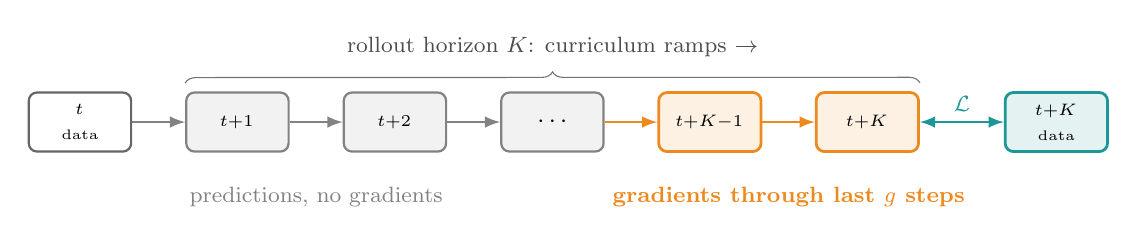
\begin{tikzpicture}[font=\small, >=latex, x=1cm, y=1cm,
    s/.style={rounded corners=3pt,draw=black!60,line width=0.8pt,fill=white,
              align=center,inner sep=4pt,minimum height=0.75cm,minimum width=1.3cm},
    sp/.style={rounded corners=3pt,draw=rollpred,line width=0.8pt,fill=black!5,
               align=center,inner sep=4pt,minimum height=0.75cm,minimum width=1.3cm},
    sg/.style={rounded corners=3pt,draw=rollgrad,line width=1pt,fill=rollgrad!12,
               align=center,inner sep=4pt,minimum height=0.75cm,minimum width=1.3cm},
    tr/.style={rounded corners=3pt,draw=rolltgt,line width=1pt,fill=rolltgt!12,
               align=center,inner sep=4pt,minimum height=0.75cm,minimum width=1.3cm}]

  %% Rollout chain: data -> no-grad predictions -> grad steps -> target
  \node[s]  (x0) at (0,0)     {$\state_t$\\[-1pt]{\tiny data}};
  \node[sp] (x1) at (2.0,0)   {$\shat_{t+1}$};
  \node[sp] (x2) at (4.0,0)   {$\shat_{t+2}$};
  \node[sp] (x3) at (6.0,0)   {$\cdots$};
  \node[sg] (x4) at (8.0,0)   {$\shat_{t+K-1}$};
  \node[sg] (x5) at (10.0,0)  {$\shat_{t+K}$};
  \node[tr] (xt) at (12.4,0)  {$\state_{t+K}$\\[-1pt]{\tiny data}};

  \draw[->,line width=0.9pt,rollpred] (x0) -- (x1);
  \draw[->,line width=0.9pt,rollpred] (x1) -- (x2);
  \draw[->,line width=0.9pt,rollpred] (x2) -- (x3);
  \draw[->,line width=0.9pt,rollgrad] (x3) -- (x4);
  \draw[->,line width=0.9pt,rollgrad] (x4) -- (x5);
  \draw[<->,line width=0.9pt,rolltgt] (x5) -- node[above,font=\footnotesize]{$\mathcal{L}$} (xt);

  %% Curriculum brace above the rollout
  \draw[decorate,decoration={brace,amplitude=4pt,raise=3pt},black!55]
    (x1.north west) -- (x5.north east)
    node[midway,above=9pt,font=\footnotesize,text=black!70]
    {rollout horizon $K$: curriculum ramps $\kzero \to \kmax$};

  %% Group labels below
  \node[text=rollpred,font=\footnotesize] at (3.0,-0.95)
    {predictions, no gradients};
  \node[text=rollgrad,font=\footnotesize\bfseries] at (9.0,-0.95)
    {gradients through last $g$ steps};

\end{tikzpicture}
